\documentclass[10pt,a4paper]{article}
\usepackage[latin1]{inputenc}
\usepackage{amsmath}
\usepackage{amsfonts}
\usepackage{amssymb}
\usepackage{hyperref}
\usepackage{graphicx}
\usepackage{mhchem}
\usepackage[lastexercise]{exercise}
\usepackage{enumitem}
\usepackage{float}
\usepackage{makecell}
\renewcommand\theadfont{\bfseries}

\newenvironment{exercises}{\begin{description}[style=nextline]}{\end{description}}


\begin{document}
\title{Networker's guide to decibels}
\author{Christian F�ssler, Institute for networked solutions}
\maketitle
\section{Motivation}
Why shall we bother with logarithms rather than just use linear values? Numbers in the logarithmic domain have the great advantage of being easy to manipulate.
\begin{itemize}
	\item Multiply numbers: add their logarithms\\
	$log(10 \cdot 20) = log(10) + log(20)$
	\item Divide numbers: subtract their logarithms\\
	$log(\frac{10}{20}) = log(10) - log(20)$
\end{itemize}
\subsection{Example}
Multiply $100$ with $12122$. Either by using linear numbers or their logarithmic representation. \\
\subsubsection{Linear}
\begin{equation}
\begin{aligned}
100 \cdot 12122 = 13358444
\end{aligned}
\end{equation}


\subsubsection{Logarithmic}
		\begin{equation}
		\begin{aligned}
		log_{10}(100 \cdot 12122) = {} &   log_{10}(100) + log_{10}(12122) \\
		= {} &  2 + log_{10}(12122)
		\end{aligned}
		\end{equation}

To get the result of $2 + log_{10}(12122)$ one has to use a lookup table, so called logarithm tables, or use a calculator. The advantage of this scheme over multiplying the numbers directly is, that these logarithm tables are relatively small compared to tables which would contain all possible multiplications.

\section{Conversion}
$$	N = 10^{\mathit{dB} /10}$$
$$ \mathit{dB} = 10\cdot log_{10}(N)$$
\begin{description}
	\item[$N$] a linear number
	\item[$\mathit{dB}$] Measure on a logarithmic scale
\end{description}

\subsection{Examples}
An antenna has a gain factor of 100, i.e it does amplify the output power 100 times. We can also say it has a 20-dB gain, because:
$$10 \cdot log_{10}(100) = 10 \cdot 2 = 20 \mathit{dB} $$

\subsection{Attenuation and Gain}
To model signal loss, the most natural way is to explain the loss by multiplying the orignal signal with a factor. For instance, if the sender sends the signal with power $log_{10}(N)$ the receiver receives the signal with power $c \cdot log_{10}(N)$. If the receiver only receives a hundreth of it, this would be $\frac{1}{100}\cdot log_{10}(N)$, or expressed with logarithms a loss of $20 \mathit{dB}$. A loss simply has a negative sign (remember division by subtracting logarithms). Now you should see that this makes mental maths very easy.

\subsection{Calculation scheme}
You might wonder how you calculate the $\mathit{dB}$ values, such as the $log_{10}(12122)$ in the example above. The answer is: you simply do not. Manufacturers usually already list characteristics with $\mathit{dB}$ values. For example if you buy an antenna, there is a figure which tells you the gain factor in decibels. The calculation scheme is usually start-off your calculations with $\mathit{dB}$ values and do the conversion back to linear values as late as possible , but this is usually not needed at all.

\subsection{Link model / Link budget}
Transmission paths are ususally modelled as one-way paths. This means a sending station transmits (TX) to a receiving station, which receives (RX) the signal. Simple as that. For back communication in the opposite direction, it follows the same scheme, only the roles change. Thus, the communication paths are regarded as independent.
Once a signal is generated in the sender, it passes several stages until it arrives at the receiver. By passing these stages it either experiences gain or attenuation. For example a stage in a wireless network is the propagation through air. In wired networks propagation through copper or fibre. These stages are modelled as a sum of logarithms.
Common stages are:

\begin{description}
	\item[Modulator output $P_{TX}$] the raw signal generated by a device ( $\mathit{dBm}$)
	\item[TX antenna gain $G_{AntTX}$] gain of the signal by the transmitting antenna ($\mathit{dB}$)
	\item[Path loss $PL$] the attenuation that occurs on the air ($\mathit{dB}$). This is usually frequency dependent ($\mathit{dB}$).
	\item[RX antenna gain $G_{AntRX}$] gain of the signal by the receiving antenna ($\mathit{dB}$)
\end{description}

To be a little bit more precise, there are some other losses involved. For example in the connection cable from the modulator output to the antenna. Also every plug adds to the attenuation. Manufacturers usually list these attenuations in the datasheets.
\subsubsection{Link budget}
Now you can do your path calculations by simply add up all your gains and attenuation values. The resulting equation is called the link-budget. For example:

\begin{equation}
\label{equ:pathf}
P_{TX} + G_{AntTX}\hspace{1.5em}-
{PL}\hspace{1.5em} + G_{AntRX} = P_{RX}
\end{equation}
\begin{equation}
\label{equ:path}
\underbrace{20 \mathit{dBm} + 3 \mathit{dB}}_\text{power of sender}\hspace{1.5em}
 \underbrace{- 80 \mathit{dB}}_\text{path loss} \hspace{1.5em}
 \underbrace{+ 3 \mathit{dB}}_\text{gain of receiver}  = \underbrace{-54 \mathit{dBm}}_\text{received power}
\end{equation}

This is where another important concept comes in place: the receiver sensitivity. This is the lowest $\mathit{dB}$ level at which the receiver is able to successfully receive the signal. For example if the receiver sensitivity is $-90\mathit{dBm}$, the receiver would be able to successfully receive the signal calculated in \autoref{equ:path} ($-54$ is bigger than $-90$).

\section{dBm}
Whereas $\mathit{dB}$ values only express a ratio, $\mathit{dBm}$ express a ratio to a fixed base of 1$\mathit{mW}$. For example, if you have a sender that has an output power $P_{TX}$ of 1 Watt, it has a $\mathit{dBm}$ output value of:
\begin{equation}
\mathit{dBm} = 10 \cdot log_{10}(\frac{P_{TX}}{1 \mathit{mW}}) = 10 \cdot log_{10}(\frac{1000 \mathit{mW}}{1 \mathit{mW}}) = 30 \mathit{dBm}
\end{equation}

\section{dBi}
Like $\mathit{dBm}$, $\mathit{dBi}$ is a value with a fixed base. But the base is not a fixed number, it is a theoretical concept. $\mathit{dBi}$ are used to express antenna gains. The base reference is the behaviour of an isotropic antenna. Isotropic simply means its transmission characteristic is the same in all directions. You can conceive it as transmitting as a sphere around the antenna.
Isotropic antennas are ideal in terms of equal power distribution, but this such an antenna does not exist. $\mathit{dBi}$ measure the antenna gain compared to this ideal antenna. Note that the maximal output power of an antenna $P_{TX}$ is usually given by regulations. So how can you achieve a wider range with the given power? Simply direct the beam in the particular direction you need it, and do not send it in other directions. By this you bring together more power, but only in one direction. The directionality loss is the trade-off.

\section{Antennas}
As soon as it comes to wireless signal transmission one has to consider beam forming and radiation patterns. As opposed to the propagation direction in cables, which is given. As a simplification you can imagine electromagnetic waves used by wireless technology just as form of non visible light. There exist two types of antennas: omnidirectional and directional. The third type, the isotropic antenna, is only a hypothetical model and does not exist in the real world (except the sun).
For detailed information on the different antenna types and radiation patterns have a look at this \href{http://www.cisco.com/c/en/us/products/collateral/wireless/aironet-antennas-accessories/prod_white_paper0900aecd806a1a3e.html}{article on antennas from Cisco}

\section{EIRP}
Equivalent isotropically radiated power. Is the  $\mathit{dBm}$ value that is actually leaving the antenna. One has to take into account the $P_{TX}$ of the sender, any attenuation by cables, plugs, amplifiers and the antenna gain. This is usually the value that is given by radio regulations. To comply with this regulations lies in the responsibility of the device operator. The output power of a transmitter is usually adjustable to help to compensate for this losses that occur on the way to the antenna. 

\subsection{isotropic}
The radio waves are radiated with the same intensity in all directions. Imagine this as a sphere.
\begin{figure}[H]
	\centering
	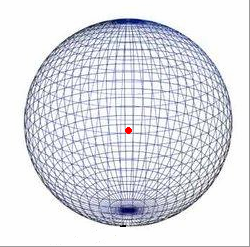
\includegraphics[scale=0.8]{isotropic-pattern.png}
	\caption{Isotropic radiation}
	\label{fig:awesome_image}
\end{figure}
\subsection{omnidirectional}
Omnidirectional antennas radiate signals uniformly in one plane in all directions. Imagine this as a Donut. The radiation in the elevation pane is not as big as in the azimut pane.
\begin{figure}[H]
	\centering
	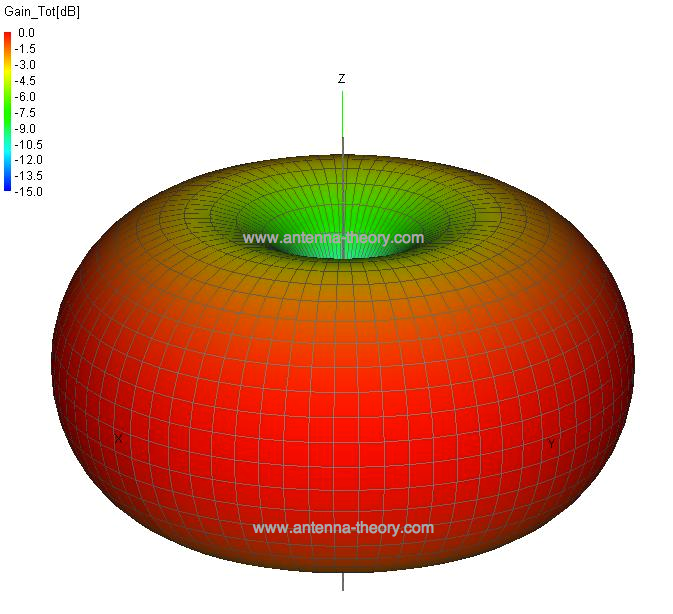
\includegraphics[scale=0.3]{omni-pattern.png}
	\caption{Omnidirectional radiation}
	\label{fig:awesome_image}
\end{figure}
\subsection{directional}
Directional antennas radiate their power especially in one direction. Usually the beam is formed like a baseball bat in the desired direction.
\begin{figure}[H]
	\centering
	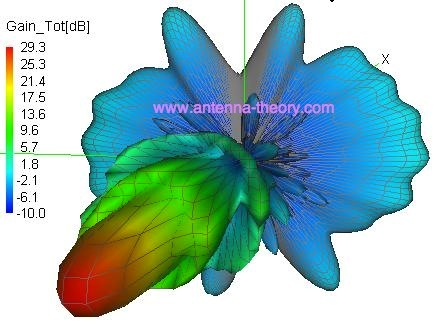
\includegraphics[scale=0.3]{directional-pattern.jpg}
	\caption{Directional radiation}
	\label{fig:awesome_image}
\end{figure}

\section{Summary}
\begin{description}
	\item[$\mathit{dB}$] Expresses a factor
	\item[$\mathit{dBm}$] Expresses power in milliwats
	\item[$\mathit{dBi}$] Antenna gain compared to a hypothetically lossless isotropic antenna
\end{description}

\section{Exercises}
\begin{exercises}
	\item[Convert 4W into $\mathit{dBm}$]	
		\begin{equation}
		\begin{aligned}
		4W = {} &  4000 \;\mathit{mW} \\
		10 \cdot log_{10}(4000) = {} & 36 \;\mathit{dBm}
		\end{aligned}
		\end{equation}
	\item[Convert 8W into $\mathit{dBm}$]
		\begin{equation}
		\begin{aligned}
		8W = {} &  8000 \;\mathit{mW} \\
		10 \cdot log_{10}(8000) = {} & 39 \;\mathit{dBm}
		\end{aligned}
		\end{equation}
		\item[Link budget calculation]
		Consider the following situation: A receiver has a  $P_{TX}$ of $20 \mathit{dBm}$, with an directional antenna attached at both the receiver and transmitter with a gain of $+5\mathit{dBi}$, the atmospheric loss is $20 \mathit{dB}$, and the receiver's sensitivity is  $-140\mathit{dB}$. Which signal strength would the receiver receive? And would it be able to successfully decode the signal?
		\begin{equation}
		\begin{aligned}
		P_{RX} = {} &20\;\mathit{dBm} + 5\;\mathit{dBi}- 80\;\mathit{dB}+5\;\mathit{dBi}\\
		P_{RX} = {} &-50\;\mathit{dBm}
		\end{aligned}
		\end{equation}
		$-50\;\mathit{dB}$ is way bigger than $-140\;\mathit{dB}$, this means the receiver can successfully decode the signal.
\end{exercises}

\section{Typical figures}
\begin{table}[h]
\begin{tabular}{|l|l|p{10cm}|}
	\hline  \thead{Power level} & \thead{Power } &\thead{Application } \\ 
	\hline  $80\;\mathit{dBm}$& $100\;\mathit{kW}$ & FM Radio station\\ 
	\hline  $60\;\mathit{dBm}$& $1000\;\mathit{W}$ & Microwave oven\\ 
	\hline  $33\;\mathit{dBm}$& $2\;\mathit{W}$ & Maximum output from a GSM850/900 mobile phone\\
	\hline  $23\;\mathit{dBm}$& $200\;\mathit{mW}$ & EEE 802.11n Wireless LAN  in 5 GHz subband\\
		\hline  $20\;\mathit{dBm}$& $100\;\mathit{mW}$ & 
		IEEE 802.11b/g Wireless LAN in the 2.4 GHz band\newline Bluetooth Class 1\\
	\hline  $10\;\mathit{dBm}$& $10\;\mathit{mW}$ & 
	Bluetooth Low Energy\newline LoRa\\ 
	\hline
	
\end{tabular} 
\caption{Typical power levels (source: wikipedia.org)}

\end{table}

\end{document}
